%@TheDoctorRAB
%standard white paper/preproposal format
%
%%%%%
%
%REFERENCES
%
%neup.bst - numbered citations in order of appearance, short author list with et al in reference section
%nsf.bst - numbered citations in order of appearance, full author list in references section
%standard.bst - citations with author last name with et al for more than 2 authors; full author list in references section
%ans.bst is for ANS only. 
%
%author = {Lastname, Firstname and Lastname, Firstname and Lastname, Firstname} for all bst formats
%bst renders the author list itself
%
%author = {{Nuclear Regulatory Commission}} if the author is an organization, institution, etc., and not people
%
%title = {{}} for all
%
%for all - use \citep{-} - [1] or (Borrelli, 2021) in the text
%standard.bst \cite{-} - Borrelli (2021) in the text
%standard.bst lists references alphabetically
%the rest list numerically
%
%
%%% slides 
%
%\citep{xxxnna} where the citation should go
%\blfootnote{\fontsize\cite{xxxnna}\fontsize\bibentry{xxxnna}} before \end{frame}
%
%
%%%%%

%%%%% presentation settings
\documentclass[aspectratio=1610,pdftex,dvipsnames,compress,xcolor={dvipsnames}]{beamer}
\usetheme{Boadilla}
\usecolortheme{seahorse}
\beamertemplatenavigationsymbolsempty
\addtobeamertemplate{footnote}{\hskip -2em}{} %pushes footnote to margin
\setbeamerfont{title}{series=\bfseries}
\setbeamertemplate{page number in head/foot}[framenumber] %just gives slide number; comment out for 1/7, 2/7...
\definecolor{BackGround}{RGB}{255,250,240}
\setbeamercolor{background canvas}{bg=BackGround}
%%%%%


%%%%% general 
%\documentclass[11pt,a4paper]{article}
%\usepackage[lmargin=1in,rmargin=1in,tmargin=1in,bmargin=1in]{geometry}
\usepackage[pagewise]{lineno} %line numbering
\usepackage{setspace}
\usepackage{ulem} %strikethrough - do not \sout{\cite{}}
\usepackage{graphicx}
\usepackage{mypythonhighlight,verbatim}
\usepackage{filecontents}
\usepackage{tablefootnote}
\usepackage{footnotehyper}
\usepackage{float}
%\usepackage{subfig}
\usepackage[yyyymmdd]{datetime} %date format
\renewcommand{\dateseparator}{.}
\graphicspath{{img/}} %path to graphics
\setcounter{secnumdepth}{5} %set subsection to nth level
\usepackage{needspace}
\usepackage[stable,hang,flushmargin]{footmisc} %footnotes in section titles and no indent; standard.bst
\usepackage[inline]{enumitem}
\setlist[itemize]{label=\textbullet}
\usepackage{boldline}
\usepackage{makecell}
\usepackage{booktabs}
\usepackage{amssymb}
\usepackage{gensymb}
\usepackage{amsmath,nicefrac}
\usepackage{physics}
\usepackage{lscape}
\usepackage{array}
\usepackage{chngcntr}
\usepackage{hyperref}
\hypersetup{colorlinks,linkcolor=black,citecolor=black,urlcolor=blue} 
%\usepackage{sectsty}
\usepackage{textcomp}
\usepackage{lastpage}
\usepackage{xargs} %for \newcommandx
\usepackage[colorinlistoftodos,prependcaption,textsize=tiny]{todonotes} %makes colored boxes for commenting
\usepackage{soul}
\usepackage{color}
\usepackage{marginnote}
\usepackage[figure,table]{totalcount}
\usepackage[capitalise]{cleveref}
\usepackage{microtype} %improves typography for pdf
\usepackage[pdftex,dvipsnames]{colortbl} %change font color
%%%%%


%%%%% tikz
\usepackage{pgf}
\usepackage{tikz} % required for drawing custom shapes
\usetikzlibrary{shapes,arrows,automata,trees}
%%%%%


%%%%% fonts
\usepackage{times}
%\renewcommand{\sfdefault}{ubuntu}
%arial - uncomment next two lines
%\usepackage{helvet}
%\renewcommand{\familydefault}{\sfdefault}
%%%%%


%%%%% references
%\usepackage[round,semicolon]{natbib} %for (Borrelli 2021; Clooney 2019) - standard.bst 
\usepackage[numbers,sort&compress]{natbib} %for [1-3] - nsf.bst, neup.bst
\setlength{\bibsep}{7pt} %sets space between references
%\renewcommand{\bibsection}{} %suppresses large 'references' heading
%\renewcommand\bibpreamble{\vspace{\baselineskip}} %sets spacing after heading if not using default references heading
%%%%%


%%%%% tables and figures
\usepackage{longtable} %need to put label at top under caption then \\ - use spacing
\usepackage{tablefootnote}
\usepackage{tabularx}
\usepackage{multirow}
\usepackage{tabto} %general tabbed spacing
\usepackage{pdfpages}
\usepackage{wrapfig} %wraps figures around text
\setlength{\intextsep}{0.00mm}
\setlength{\columnsep}{1.00mm}
\usepackage[singlelinecheck=false,labelfont=bf]{caption}
\usepackage{subcaption}
\captionsetup[table]{justification=justified,skip=5pt,labelformat={default},labelsep=period,name={Table}} %sets a space after table caption
\captionsetup[figure]{justification=justified,skip=5pt,labelformat={default},labelsep=period,name={Figure}} %sets space above caption, 'figure' format
\captionsetup[wrapfigure]{justification=centering,aboveskip=0pt,belowskip=0pt,labelformat={default},labelsep=period,name={Fig.}} %sets space above caption, 'figure' format
\captionsetup[wraptable]{justification=centering,aboveskip=0pt,belowskip=0pt,labelformat={default},labelsep=period,name={Table}} %sets space above caption, 'figure' format
%%%%%


%%%%% watermark
%\usepackage[firstpage,vpos=0.63\paperheight]{draftwatermark}
%\SetWatermarkText{\shortstack{DRAFT\\do not distribute}}
%\SetWatermarkScale{0.20}
%%%%%


%%%%% cross referencing files
%\usepackage{xr} %for revisions - will cross reference from one file to here
%\externaldocument{/path/to/auxfilename} %aux file needed
%%%%%


%%%%% toc and glossaries
\usepackage[toc,title]{appendix}
\usepackage[acronym,nomain,nonumberlist]{glossaries}
\makenoidxglossaries
%\usepackage{titlesec,titletoc}
%\renewcommand{\thepart}{ARTICLE \Roman{part}} %puts the label into the command so \thelabel will carry through
%\renewcommand{\thesection}{\arabic{section}} %puts the label into the command so \thelabel will carry through
%\titleformat{\part}{\normalfont\large\bfseries}{\thepart}{}{}[]
%\titlespacing*\part{0pt}{0.95\baselineskip}{0.75\baselineskip}
%\titleformat{\section}[runin]{\normalfont\large\bfseries}{\thesection}{-1em}{}[.]
%\titlespacing*\section{0pt}{0.65\baselineskip}{0.55\baselineskip}
%\titleformat{\subsection}[runin]{\normalfont\normalsize\bfseries}{\thesubsection}{-1em}{}[.]
%\titlespacing*\subsection{0pt}{0.50\baselineskip}{0.35\baselineskip}
%\titleformat{\paragraph}[runin]{\normalfont\normalsize\bfseries\itshape}{\theparagraph}{-1em}{}[.]
%\titlespacing*\paragraph{0pt}{0.45\baselineskip}{0.25\baselineskip}
%\titleformat{\subparagraph}[runin]{\normalfont\normalsize\itshape}{\thesubparagraph}{-1em}{}[.]
%\titlespacing*\subparagraph{0pt}{0.40\baselineskip}{0.25\baselineskip}
%\titleformat{\paragraph}[hang]{\normalfont\normalsize\bfseries}{\theparagraph}{5pt}{}[]
%\titlespacing*\paragraph{0pt}{0.50\baselineskip}{0.25\baselineskip}
%\titleformat{\subparagraph}[runin]{\normalfont\normalsize\itshape}{\thesubparagraph}{-1em}{}[.]
%\titlespacing*\subparagraph{0pt}{0.40\baselineskip}{0.20\baselineskip}
%%%%%


%%%%% editing
\newcommand{\edit}[1]{\textcolor{blue}{#1}} %shortcut for changing font color on revised text
\newcommand{\fn}[1]{\footnote{#1}} %shortcut for footnote tag
\newcommand*\sq{\mathbin{\vcenter{\hbox{\rule{.3ex}{.3ex}}}}} %makes a small square as a separator $\sq$
%\newcommand{\sk}[1]{\sout{#1}} %shortcut for default strikethrough - do not sk through citep
\newcommand\sk{\bgroup\markoverwith{\textcolor{red}{\rule[0.5ex]{1pt}{1pt}}}\ULon} %strikethrough with red line; not in \section{}
%\st{} does strikethrough using soul package but does not like acronyms
\newcommand{\blucell}{\cellcolor{aliceblue}} %use to shade in table cell
\newcommand{\grycekk}{\cellcolor{lightgray}} %use to shade in table cell
\newcommand{\whicell}{\cellcolor{antiquewhite}} %use to shade in table cell
%%%%%


%%%%% colors
%http://latexcolor.com/
%https://en.wikibooks.org/wiki/LaTeX/Colors#:~:text=black%2C%20blue%2C%20brown%2C%20cyan,be%20available%20on%20all%20systems.
\definecolor{aliceblue}{rgb}{0.94, 0.97, 1.0}
\definecolor{antiquewhite}{rgb}{0.98, 0.92, 0.84}
\definecolor{lightmauve}{rgb}{0.86, 0.82, 1.0}
\definecolor{brilliantlavender}{rgb}{0.96, 0.73, 1.0}
\definecolor{brandeisblue}{rgb}{0.0, 0.44, 1.0}
\definecolor{darkmidnightblue}{rgb}{0.0, 0.2, 0.4}

\newcommand{\x}{\cellcolor{aliceblue}} %use to shade in table cell
\newcommand{\y}{\cellcolor{lightgray}} %use to shade in table cell
\newcommand{\z}{\cellcolor{antiquewhite}} %use to shade in table cell
%%%%%


%%%%% acronyms
\newcommand{\acf}{\acrfull} %full acronym
\newcommand{\acl}{\acrlong} %long acronym
\newcommand{\acs}{\acrshort} %short acronym

\newcommand{\acfp}{\acrfullpl} %full acronym plural
\newcommand{\aclp}{\acrlongpl} %long acronym plural
\newcommand{\acsp}{\acrshortpl} %short acronym plural
%%%%%


%%%%% todonotes
\newcommandx{\cmt}[2][1=]{\todo[author=\textbf{STRUCTURE},tickmarkheight=0.15cm,linecolor=red,backgroundcolor=red!25,bordercolor=black,#1]{#2}}
\newcommandx{\con}[2][1=]{\todo[author=\textbf{CONTENT},tickmarkheight=0.15cm,linecolor=brilliantlavender,backgroundcolor=brilliantlavender,bordercolor=black,#1]{#2}}
\newcommandx{\rab}[2][1=]{\todo[noline,author=\textbf{RAB},backgroundcolor=Plum!25,bordercolor=black,#1]{#2}}


%\newcommandx{\jon}[2][1=]{\todo[noline,author=\textbf{ATTN: Johnson},backgroundcolor=blue!25,bordercolor=black,#1]{#2}}
%\newcommandx{\han}[2][1=]{\todo[noline,author=\textbf{ATTN: Haney},backgroundcolor=OliveGreen!25,bordercolor=black,#1]{#2}}
%\newcommandx{\rab}[2][1=]{\todo[author=\textbf{RAB},tickmarkheight=0.15cm,linecolor=Plum,backgroundcolor=Plum!25,bordercolor=black,#1]{#2}}
%\newcommandx{\han}[2][1=]{\todo[author=\textbf{ATTN: Haney},tickmarkheight=0.15cm,linecolor=OliveGreen,backgroundcolor=OliveGreen!25,bordercolor=OliveGreen,#1]{#2}}
%\newcommandx{\jon}[2][1=]{\todo[author=\textbf{ATTN: Johnson},tickmarkheight=0.15cm,linecolor=blue,backgroundcolor=blue!25,bordercolor=blue,#1]{#2}}


% highlighting 
\DeclareRobustCommand{\hlc}[1]{{\sethlcolor{LimeGreen}\hl{#1}}}
\makeatletter
    \if@todonotes@disabled
    \newcommand{\hlh}[2]{#1}
    \else
    \newcommand{\hlh}[2]{\han{#2}\hlc{#1}}
    \fi
    \makeatother

\DeclareRobustCommand{\hld}[1]{{\sethlcolor{CornflowerBlue}\hl{#1}}}
\makeatletter
    \if@todonotes@disabled
    \newcommand{\hlj}[2]{#1}
    \else
    \newcommand{\hlj}[2]{\jon{#2}\hld{#1}}
    \fi
    \makeatother

\DeclareRobustCommand{\hlf}[1]{{\sethlcolor{lightmauve}\hl{#1}}}
\makeatletter
    \if@todonotes@disabled
    \newcommand{\hlb}[2]{#1}
    \else
    \newcommand{\hlb}[2]{\rab{#2}\hlf{#1}}
    \fi
    \makeatother
%%%%%


%%%%% table alignments
\newcolumntype{L}[1]{>{\raggedright\let\newline\\\arraybackslash\hspace{0pt}}m{#1}} %uses \raggedright with m,p{} in table column
\newcolumntype{C}[1]{>{\centering\let\newline\\\arraybackslash\hspace{0pt}}m{#1}} %uses \raggedright with m,p{} in table column
\newcolumntype{R}[1]{>{\raggedleft\let\newline\\\arraybackslash\hspace{0pt}}m{#1}} %uses \raggedright with m,p{} in table column
%%%%%


%%%%% table contents
\makeatletter
\renewcommand\tableofcontents{%
    \@starttoc{toc}%
}
\makeatother

\makeatletter
\renewcommand\listoffigures{%
    \@starttoc{lof}%
}
\makeatother

\makeatletter
\renewcommand\listoftables{%
    \@starttoc{lot}%
}
\makeatother

\makeatletter
\newcommand*\ftp{\fontsize{16.5}{17.5}\selectfont}
\makeatother
%%%%%


%%%%% user commands
\newcommand\blfootnote[1]{%
  \begingroup
  \renewcommand\thefootnote{}\footnote{#1}%
  \addtocounter{footnote}{-1}%
  \endgroup
}

\makeatletter
\renewcommand{\@biblabel}[1]{#1.\hfill} %bibliography ordered list has numbers left flush
\makeatother
%%%%%

%%%%% archived section commands - use titlesec
%\makeatletter
%\renewcommand\section{%
%    \@startsection{section}{1}{\z@ }{0.50\baselineskip}{0.25\baselineskip}
%    {\large \normalfont \bfseries}}%

%\makeatletter
%\renewcommand\paragraph{%
%    \@startsection{paragraph}{4}{\z@ }{0.55\baselineskip}{-1em}
%    {\normalfont \normalsize \bfseries}}%

%\makeatletter
%\renewcommand\subparagraph{%
%    \@startsection{subparagraph}{5}{\z@ }{0.40\baselineskip}{-1em}
%    {\normalfont \normalsize \itshape }}%

%\makeatletter
%\renewcommand\subsection{%
%    \@startsection{subsection}{2}{\z@ }{0.45\baselineskip}{0.25\baselineskip}
%    {\large \normalfont \bfseries}}%
%%%%%


%%%%% header and footer
%\usepackage{fancyhdr}
%\pagestyle{fancy}
%\fancyhf{} %move page number to bottom right
%\renewcommand{\headrulewidth}{0pt} %set line thickness in header; uncomment as is to remove line
%\lhead{\scriptsize Name}
%\lhead{\scriptsize PNUCENE-D-22-xxxxx}
%\chead{\scriptsize \textit{PhD White Paper Project Proposal}}
%\rhead{\scriptsize \today}
%\rfoot{\thepage}
%%%%%


%%%%%%% citations
%\begin{filecontents}{references.bib}
%\end{filecontents}
%%%%%%%


%%%%% acronyms
% alphabetical ordering is automated
\newacronym{nrs}{NRHES}{Nuclear Renewable Hybrid Energy System}
\newacronym{ahp}{AHP}{Analytical Hierarchy Process}
\newacronym{inl}{INL}{Idaho National Laboratory}
\newacronym{orl}{ORNL}{Oak Ridge National Laboratory}
\newacronym{anl}{ANL}{Argonne National Laboratory}
\newacronym{npp}{NPP}{Nuclear Power Plant}
\newacronym{smr}{SMR}{Small Modular Reactor}
\newacronym{ump}{UAMPS}{Utah Associated Municipal Power Systems}
\newacronym{nus}{NuScale}{NuScale Power, LLC}
\newacronym{nrc}{NRC}{United States Nuclear Regulatory Commission}
\newacronym{epri}{EPRI}{Electric Power Research Institute}
\newacronym{nerc}{NERC}{North American Electric Reliability Corporation}
\newacronym{ci}{CI}{Consistency Index}
\newacronym{cr}{CR}{Consistency Ratio}
\newacronym{htse}{HTSE}{High Temperature Steam Electrolysis}
\newacronym{lwr}{LWR}{Light Water Reactor}
\newacronym{eia}{EIA}{U.S. Energy Information Administration}
\newacronym{oer}{OER}{Online Educational Resource}
\newacronym{lms}{LMS}{Learning Management System}
\newacronym{cps}{CPS}{Cyber-Physical Systems}
\newacronym{nsf}{NSF}{National Science Foundation}
\newacronym{wsc}{WSC}{Western Services Corporation}
\newacronym{cae}{CAES}{Center for Advanced Energy Studies}
\newacronym{hsl}{HSSL}{Human System Simulation Laboratory}
\newacronym{pwr}{PWR}{Pressurized Water Reactor}
\newacronym{bwr}{BWR}{Boiling Water Reactor}
\newacronym{roi}{ROI}{Return on Investment}
\newacronym{ic}{I\&C}{Instrumentation \& Controls}
\newacronym{mwe}{MWe}{Megawatts-electric}
\newacronym{ics}{ICS}{Industrial Control Systems}
\newacronym{sca}{SCADA}{Supervisory Control and Data Acquisition}
\newacronym{ip}{IP}{Internet Protocol}
\newacronym{udp}{UDP}{User Datagram Protocol}
\newacronym{tva}{TVA}{Tennessee Valley Authority}
\newacronym{plc}{PLC}{Programmable Logic Controller}
\newacronym{vfd}{VFD}{Variable Frequency Drive}
\newacronym{khp}{KHNP}{Korean Hydro \& Nuclear Power Co., Ltd}
\newacronym{onl}{ORNL}{Oak Ridge National Laboratory}
\newacronym{jcp}{JCPOA}{Joint Comprehensive Plan of Action}
\newacronym{mim}{MITM}{Man in the Middle}
\newacronym{dos}{DDoS}{Distributed Denial of Service}
\newacronym{tcp}{TCP/IP}{Transmission Control Protocol/Internet Protocol}
\newacronym{dnp}{DNP3}{Distributed Network Protocol 3}
\newacronym{pra}{PRA}{Probabilistic Risk Assessment}
\newacronym{cs}{CS}{Critical System}
\newacronym{loc}{LOCA}{Loss of Coolant Accident}
\newacronym{hmi}{HMI}{Human Machine Interface}
\newacronym{pha}{PHA}{Preliminary Hazards Analysis}
\newacronym{bol}{BOL}{Beginning-of-Life}
\newacronym{eol}{EOL}{End-of-Life}
\newacronym{mol}{MOL}{Middle-of-Life}
\newacronym{imu}{IMUNES}{Integrated Multiprotocol Network Emulator/Simulator}
\newacronym{ccc}{CCC}{Computing Community Consortium}
\newacronym{neu}{NEUP}{Nuclear Energy University Program}
\newacronym{doe}{DOE}{United States Department of Energy}
\newacronym{nei}{NEI}{Nuclear Energy Institute}
\newacronym{nit}{NITRD}{Networking Information Technology Research \& Development Program}
\newacronym{rcs}{RCS}{Reactor Cooling System}
\newacronym{con}{IC}{Initial Condition}
\newacronym{csi}{CSIS}{Center for Strategic \& International Studies}
\newacronym{pcap}{PCAP}{packet capture file}
\newacronym{dc}{DC}{Direct-Current}
\newacronym{ac}{AC}{Alternating-Current}
\newacronym{iff}{UIIF}{Idaho Falls Center for Higher Education}
\newacronym{snl}{SNL}{Sandia National Laboratory}
\newacronym{cie}{CIE}{Cyber-Informed Engineering}
\newacronym{cds}{CRDS}{Control Rod Drive System}
\newacronym{cdm}{CRDM}{Control Rod Drive Mechanism}
\newacronym{fma}{FMEA}{Failure Modes \& Effects Analysis}
\newacronym{rpn}{RPN}{Risk Priority Number}
\newacronym{scr}{SCR}{silicon controller rectifier}
\newacronym{hvc}{HVAC}{Heating, Ventilation \& Air Conditioning}
\newacronym{ttb}{TTB}{Time-to-Boil}
\newacronym{sis}{SIS}{Safety Instrumented System}
\newacronym{ui}{UI}{University of Idaho}
\newacronym{ala}{ALARA}{As Low As Reasonably Achievable}
\newacronym{pdf}{PDF}{Probability Density Function}
\newacronym{cdf}{CDF}{Cumulative Distribution Function}
\newacronym{osa}{OSHA}{Occupational Safety and Health Administration}
\newacronym{haz}{HAZOP}{Hazard \& Operability Analysis}
%\newacronym{}{}{}
%%%%%

%%%%% spacing
%\onehalfspacing %linespacing
%\setstretch{1.05} %linespacing
%\spacing{1.25} %equivalent to 1.5 line spacing in Word
%%%%%


%%%%% linenumbering
%\linenumbers %toggle line numbers
%\pagewiselinenumbers %reset line numbers on new page
%\modulolinenumbers[1] %line numbering interval
%%%%%


%%%%% title page
\addtocounter{framenumber}{-1} %does not count the title slide in the slide count
\title[NE529 -- Risk Assessment]{NE529\\RISK ASSESSMENT\\\acl{fma}\\4}
\author[@TheDoctorRAB]{R. A. Borrelli}
\institute[]{
    \acl{ui}\\
    \vspace{0.10in}
    
\includegraphics[width=0.20\textwidth]{ne-logo.png}
    }
\date{\acl{iff}}
%%%%%


\begin{document}


%%%%% title page with no footer
{
    \setbeamertemplate{footline}{}
    \begin{frame}
        \titlepage
    \end{frame}
}
%%%%%


\begin{frame}{Learning objectives}
    \begin{enumerate}[series=outerlist,topsep=0pt,itemsep=21pt,leftmargin=*,label=(\arabic*)]
        \item[]Chapter 11 in book
        \item[]Explain and analyze failures for process, system, product in detail
        \item[]My m/o is to use this time to show the concepts with my examples
        \item[]See case studies and literature in the \href{https://uidaho.pressbooks.pub/riskassessment/}{\acs{oer}} to supplement the lecture
        \item[]Choose what is most interesting and relevant to you
        \item[]Immersive critical thinking -- always the three questions 
    \end{enumerate}
\end{frame}


\begin{frame}{Learning nodes}
    \begin{columns}[t]

        \begin{column}{0.50\textwidth}
            \begin{enumerate}[series=outerlist,topsep=0pt,itemsep=1pt,leftmargin=*,label=(\arabic*)]
                \item[]\textbf{What \acs{fma} is}
                    \vspace{0.10in}
                \item[]\textbf{\acs{fma} definitions}
                    \vspace{0.10in}
                \item[]\textbf{Utility of \acs{fma}}
            \end{enumerate}
        \end{column}

        \begin{column}{0.50\textwidth}
            \begin{enumerate}[series=outerlist,topsep=0pt,itemsep=1pt,leftmargin=*,label=(\arabic*)]
                \item[]\hfill\textbf{\acs{fma} procedure}
                \item[]\hfill Construct flow chart
                \item[]\hfill Define failure modes  
                \item[]\hfill Establish failure effects  
                \item[]\hfill Failure mode matrix examples  
                \item[]\hfill Evaluate severity  
                \item[]\hfill Estimate failure frequency  
                \item[]\hfill Calculate \acf{rpn}
                    \vspace{0.10in}
                \item[]\hfill\textbf{Root cause analysis}
                    \vspace{0.10in}
                \item[]\hfill\textbf{Mitigation}
            \end{enumerate}
        \end{column}

    \end{columns}
\end{frame}


\begin{frame}{It's really hard to quantify risk}
    \begin{enumerate}[series=outerlist,topsep=0pt,itemsep=21pt,leftmargin=*,label=(\arabic*)]
        \item[]\acs{pra} wasn't `invented' until there were 2-ish decades of operational data
        \item[]Getting any data cohorts for an \acs{fma} is ideal but probably difficult 
        \item[]Can use related historical or similarly accident data
    \end{enumerate}
\end{frame}


\begin{frame}{Draw upon expert judgement and best estimates}
    \begin{enumerate}[series=outerlist,topsep=0pt,itemsep=21pt,leftmargin=*,label=(\arabic*)]
        \item[]Can use a \href{https://uidaho.pressbooks.pub/riskassessment/chapter/failure-rates/}{Delphi} technique
        \item[]Iterative way to develop consensus about something
    \end{enumerate}
\end{frame}


\begin{frame}[plain]{}
    \centering\LARGE\textbf{What \acs{fma} is}
\end{frame}


\addtocounter{framenumber}{-1}
\begin{frame}{\acs{fma} helps to develop a firm understanding of what a failure is prior to risk analysis}
    \begin{enumerate}[series=outerlist,topsep=0pt,itemsep=11pt,leftmargin=*,label=(\arabic*)]
        \item[]Detailed document that identifies ways in which process/product fails
        \item[]Or does not meet critical requirements
        \item[]Inductive -- Sherlock Holmes  
        \item[]Bottom up, forward search approach
        \item[]Living document that lists all the possible causes of failure
        \item[]Items can be generated to determine types of controls/changes in procedures 
        \item[]Systematic way to identify and prevent problems in processes and products before they occur  
        \item[]Design driven approach
    \end{enumerate}
\end{frame}


\begin{frame}{\acs{fma} is a proactive tool to assist in new service design or enhancement of existing processes}
    \begin{enumerate}[series=outerlist,topsep=0pt,itemsep=21pt,leftmargin=*,label=(\arabic*)]
        \item[]What was the purpose of the \acs{pha}?
        \item[]How will this relate?
        \item[]\acs{fma} might be more conducive when dealing with monetary loss
        \item[]Most common for assessment technique at initial stages of system development
        \item[]Maximize design life
    \end{enumerate}
\end{frame}


\begin{frame}[plain]{}
    \centering\LARGE\textbf{\acs{fma} definitions}
\end{frame}


\addtocounter{framenumber}{-1}
\begin{frame}{Let's start with some definitions}
    \begin{enumerate}[series=outerlist,topsep=0pt,itemsep=1pt,leftmargin=*,label=(\arabic*)]
        \item[]\textbf{Failure mode}
        \item[]Ways in which a process can fail  
        \item[]Interrupts continuity of production  
        \item[]Loss of assets (not just money)  
        \item[]Unavailability of equipment  
        \item[]Deviation from normal operation
        \item[]Not meeting target expectations 
        \item[]Secondary defects 
            \vspace{0.10in}
        \item[]\textbf{Potential (failure) effect (consequence)}
        \item[]Result of failure mode
        \item[]Some more likely to occur than others
        \item[]Include regulatory requirements
    \end{enumerate}
\end{frame}


\begin{frame}{Let's continue with some definitions}
    \begin{enumerate}[series=outerlist,topsep=0pt,itemsep=1pt,leftmargin=*,label=(\arabic*)]
        \item[]\textbf{Risk of failure}
        \item[]Each potential effect carries risk associated with it
        \item[]Consequences
        \item[]Frequency
            \vspace{0.25in}
        \item[]\textbf{\acl{rpn}}
        \item[]Nominal value assigned to risk for each failure
    \end{enumerate}
\end{frame}


\begin{frame}[plain]{}
    \centering\LARGE\textbf{Can results from a \acs{pha} be applied?}
\end{frame}


\addtocounter{framenumber}{-1}
\begin{frame}{Why is \acs{fma} effective?}
    \begin{enumerate}[series=outerlist,topsep=0pt,itemsep=11pt,leftmargin=*,label=(\arabic*)]
        \item[]Identifies areas of failure in process, system, component, or procedure
        \item[]Effects of the process, system, component, or procedure failing
        \item[]Failure causes (common cause)
        \item[]Reducing the probability of failure  
        \item[]Improving the means of detecting the causes of failure  
        \item[]Risk ranking of failures, allowing risk informed decisions by those responsible 
        \item[]A starting point from which the control plan can be created
        \item[]Decomposition of risk -- focus on the areas where risk can be reduced
    \end{enumerate}
\end{frame}


\begin{frame}[plain]{}
    \centering\LARGE\textbf{\acs{fma} procedure}
\end{frame}


\begin{frame}[plain]{}
    \centering\LARGE\textbf{Flowchart}
\end{frame}


\addtocounter{framenumber}{-2}
\begin{frame}{Construct a detailed flow chart of the process}
    \begin{enumerate}[series=outerlist,topsep=0pt,itemsep=21pt,leftmargin=*,label=(\arabic*)]
        \item[]Multi-disciplinary participation of all those involved in the process
        \item[]Allocate plenty of time for this step
        \item[]Be as complete as possible
        \item[]Flow charting software can help (or write your own)
    \end{enumerate}
\end{frame}


\begin{frame}{}
    \begin{figure}
        \centering
        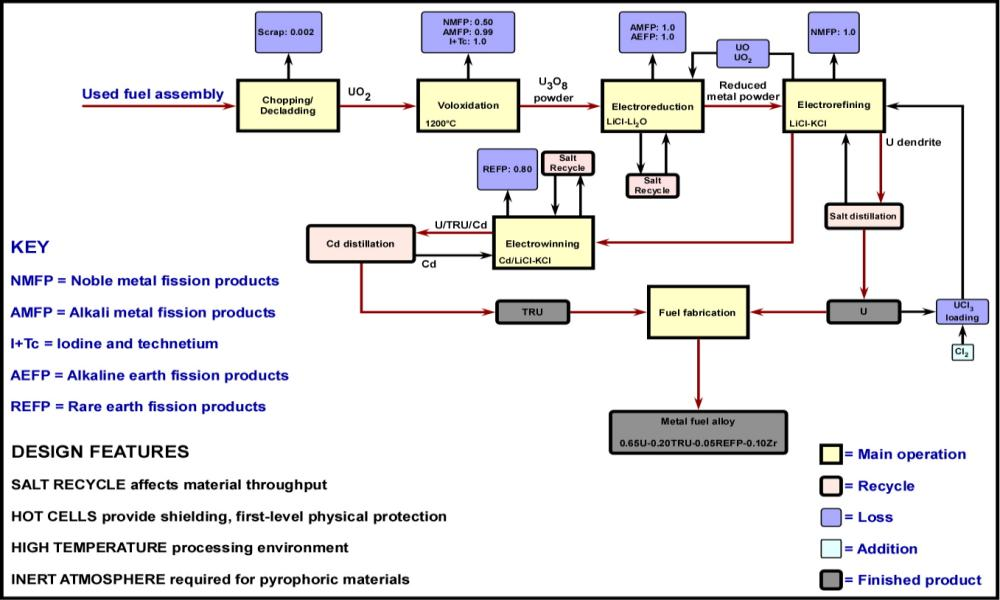
\includegraphics[width=0.80\textwidth]{pyroprocessing.flowsheet.jpg}
%        \caption{}
    \end{figure}
\end{frame}


\begin{frame}{}
    \begin{figure}
        \centering
        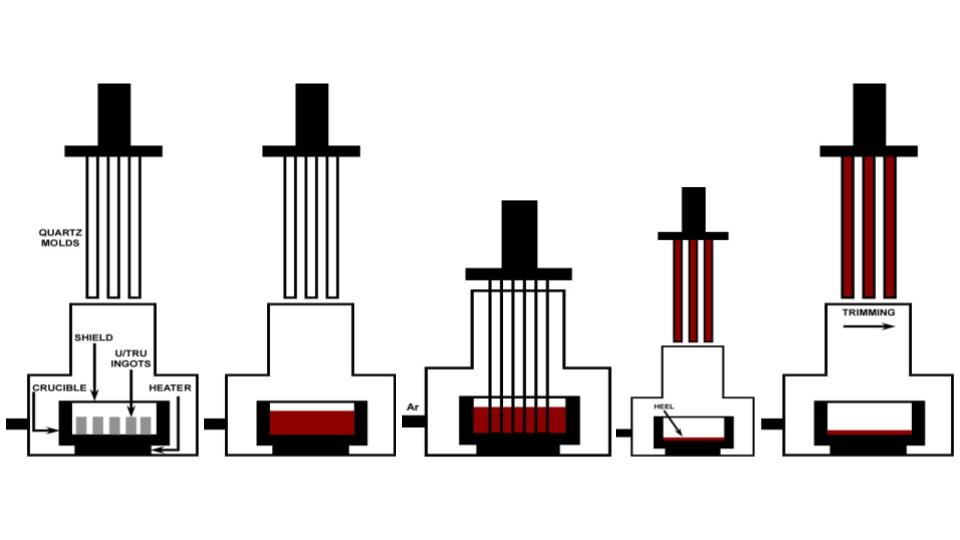
\includegraphics[width=0.80\textwidth]{fuel.fabrication.jpg}
%        \caption{}
    \end{figure}
\end{frame}


\begin{frame}{Process steps}
    \begin{figure}
        \centering
        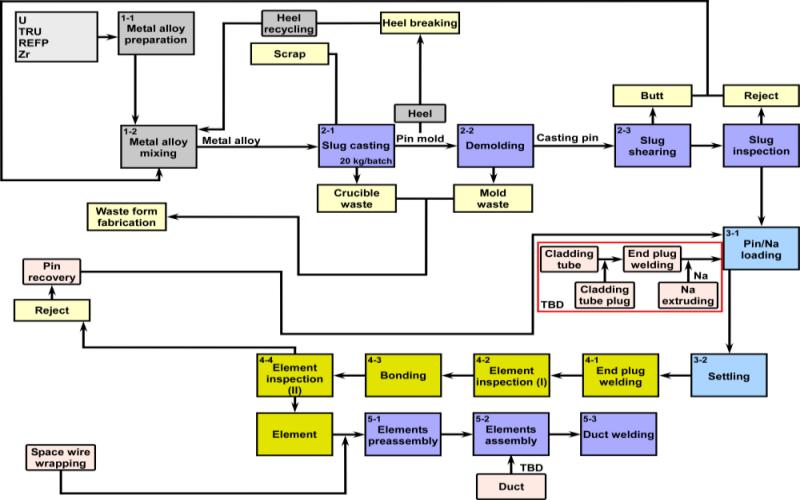
\includegraphics[width=0.80\textwidth]{fuel.fabrication.process.steps.jpg}
%        \caption{}
    \end{figure}
\end{frame}


\begin{frame}[plain]{}
    \centering\LARGE\textbf{Define failure modes}
\end{frame}


\addtocounter{framenumber}{-1}
\begin{frame}{Determine how each step could possibly fail}
    \begin{enumerate}[series=outerlist,topsep=0pt,itemsep=21pt,leftmargin=*,label=(\arabic*)]
        \item[]Getting material into the crucible -- effect -- cause
        \item[]Heater fails to sufficiently melt all the metal -- effect -- cause
        \item[]Vacuum cannot be induced -- effect -- cause
        \item[]Molds get stuck or break -- effect -- cause
        \item[]Cannot remove heel -- effect -- cause
    \end{enumerate}
\end{frame}


\begin{frame}[plain]{}
    \centering\LARGE\textbf{Failure mode matrix examples}
\end{frame}


\addtocounter{framenumber}{-1}
\begin{frame}{}
    \begin{figure}
        \centering
        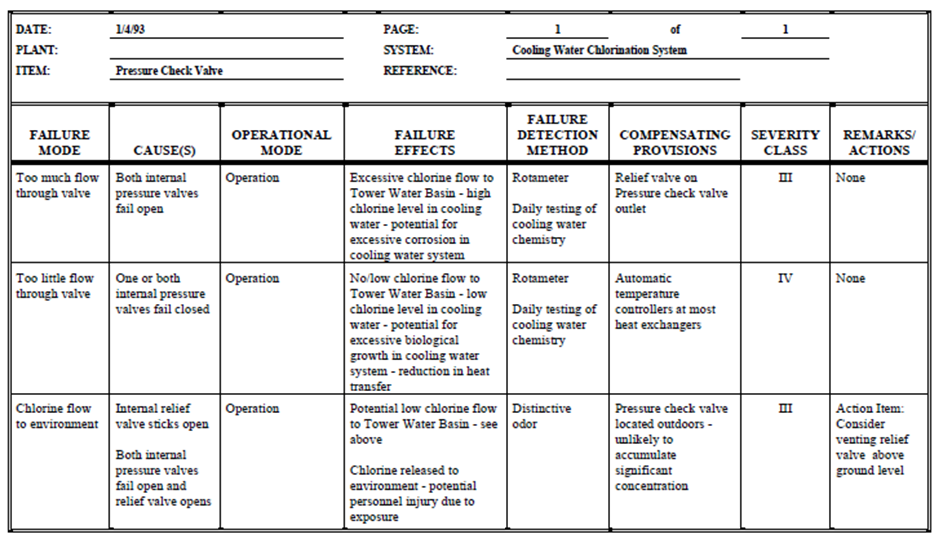
\includegraphics[width=0.80\textwidth]{pressure.check.valve.jpg}
%        \caption{}
    \end{figure}
\end{frame}


\begin{frame}{}
    \begin{figure}
        \centering
        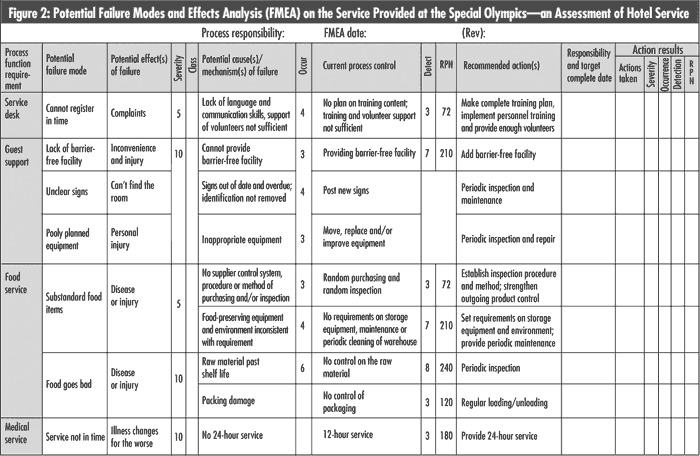
\includegraphics[width=0.80\textwidth]{hotel.service.jpg}
%        \caption{}
    \end{figure}
\end{frame}


\begin{frame}[plain]{}
    \centering\LARGE\textbf{Establish failure effects}
\end{frame}


\addtocounter{framenumber}{-1}
\begin{frame}{Determine the effects (consequences) of each possible failure}
    \begin{enumerate}[series=outerlist,topsep=0pt,itemsep=21pt,leftmargin=*,label=(\arabic*)]
        \item[]Getting material into the crucible -- crucible breaks
        \item[]Heater fails to sufficiently melt all the metal -- molds might crack; not sufficiently take up all the metal
        \item[]Vacuum cannot be induced -- no injection
        \item[]Molds get stuck or break -- big mess; liquid metal spills onto equipment
        \item[]Cannot remove heel -- replace crucible; store heel
    \end{enumerate}
\end{frame}


\begin{frame}[plain]{}
    \centering\LARGE\textbf{Evaluate severity}
\end{frame}


\addtocounter{framenumber}{-1}
\begin{frame}{Apply (or find) a Severity Rating Scale}
    \begin{enumerate}[series=outerlist,topsep=0pt,itemsep=3pt,leftmargin=*,label=(\arabic*)]
        \item[]10 -- Dangerously high -- Injury
        \item[]9 -- Extremely high -- Regulatory noncompliance
        \item[]8 -- Very high -- Equipment inoperable or unfit for use
        \item[]7 -- High -- High degree of customer dissatisfaction/bad results 
        \item[]6 -- Moderate -- Partial malfunction
        \item[]5 -- Low -- Some performance loss
        \item[]4 -- Very low -- Minor performance loss
        \item[]3 -- Minor -- Identifiable product flaws
        \item[]2 -- Very minor -- Not readily apparent product flaws
        \item[]1 -- None 
    \end{enumerate}
\end{frame}


\begin{frame}{Severity for fuel fabrication failure modes}
    \begin{enumerate}[series=outerlist,topsep=0pt,itemsep=3pt,leftmargin=*,label=(\arabic*)]
        \item[]Getting material into the crucible -- crucible breaks
        \item[]6 -- Moderate
        \item[]Failure results in subsystem or partial malfunction of the product
            \vspace{0.10in}
        \item[]Heater fails to sufficiently melt all the metal -- molds might crack; not take up all the metal
        \item[]6 -- Moderate
        \item[]Failure results in subsystem or partial malfunction of the product
            \vspace{0.10in}
        \item[]Vacuum cannot be induced -- no injection
        \item[]6 -- Moderate
        \item[]Failure results in subsystem or partial malfunction of the product
    \end{enumerate}
\end{frame}


\begin{frame}{Severity for fuel fabrication failure modes}
    \begin{enumerate}[series=outerlist,topsep=0pt,itemsep=3pt,leftmargin=*,label=(\arabic*)]
        \item[]Molds get stuck or break -- big mess; liquid metal spills onto equipment
        \item[]8 -- Very high 
        \item[]Failure renders the unit inoperable or unfit for use
            \vspace{0.10in}
        \item[]Cannot remove heel -- replace crucible; store heel
        \item[]6 -- Moderate
        \item[]Failure results in subsystem or partial malfunction of the product
            \vspace{0.10in}
        \item[]Any shutdown interrupts material flow
    \end{enumerate}
\end{frame}


\begin{frame}[plain]{}
    \centering\LARGE\textbf{Estimate failure frequency}
\end{frame}


\addtocounter{framenumber}{-1}
\begin{frame}{Estimate failure frequency with an Occurrence Rating Scale}
    \begin{enumerate}[series=outerlist,topsep=0pt,itemsep=3pt,leftmargin=*,label=(\arabic*)]
        \item[]10 -- Very high -- 1 per day or more than 3 per 10 events
        \item[]9 -- Mid -- 1 per 3,4 days or 3 per 10 events
        \item[]8 -- High -- 1 per week or 5 per 100 events
        \item[]7 -- Mid -- 1 per month or 1 per 100 events
        \item[]6 -- Moderate -- 1 per 3 months or 3 per 1000 events
        \item[]5 -- Mid -- 1 per 6 months or 1 per 10000 events
        \item[]4 -- Mid low -- 1 per year or 6 per 100000  
        \item[]3 -- Low -- 1 per 1-3 years or 6 per 1 billion events
        \item[]2 -- Mid -- 1 per 3-5 years or 2 per 1 billion events
        \item[]1 -- Remote -- 1 per $>$5 years or less than 2 per 1 billion events
    \end{enumerate}
\end{frame}


\begin{frame}{Occurrence for fuel fabrication failure modes}
    \begin{enumerate}[series=outerlist,topsep=0pt,itemsep=3pt,leftmargin=*,label=(\arabic*)]
        \item[]Getting material into the crucible -- crucible breaks
        \item[]6 -- Moderate
        \item[]1 occurrence every 3 months or 3 occurrences in 1000 events
            \vspace{0.10in}
        \item[]Heater fails to sufficiently melt all the metal -- molds might crack; not take up all the metal
        \item[]7 -- Moderate/High
        \item[]1 occurrence every month or 1 occurrence in 100 events
            \vspace{0.10in}
        \item[]Vacuum cannot be induced -- no injection
        \item[]6 -- Moderate
        \item[]1 occurrence every 3 months or 3 occurrences in 1000 events
    \end{enumerate}
\end{frame}


\begin{frame}{Occurrence for fuel fabrication failure modes}
    \begin{enumerate}[series=outerlist,topsep=0pt,itemsep=3pt,leftmargin=*,label=(\arabic*)]
        \item[]Molds get stuck or break -- big mess; liquid metal spills onto equipment
        \item[]5 -- Low/Moderate
        \item[]1 occurrence every 6 months to 1 year or 1 occurrence in 10000 events
            \vspace{0.10in}
        \item[]Cannot remove heel -- replace crucible; store heel
        \item[]7 -- Moderate/High
        \item[]1 occurrence every month or 1 occurrence in 100 events
    \end{enumerate}
\end{frame}


\begin{frame}[plain]{}
    \centering\LARGE\textbf{Calculate \acf{rpn}}
\end{frame}


\addtocounter{framenumber}{-1}
\begin{frame}{Calculate, prioritize  \acs{rpn} for each failure mode}
    \begin{enumerate}[series=outerlist,topsep=0pt,itemsep=21pt,leftmargin=*,label=(\arabic*)]
        \item[]\acs{rpn} = Severity $\times$ Occurrence
        \item[]More quantitative than prior work we've done
    \end{enumerate}
\end{frame}


\begin{frame}{\acs{rpn} for fuel fabrication failure modes}
    \begin{enumerate}[series=outerlist,topsep=0pt,itemsep=3pt,leftmargin=*,label=(\arabic*)]
        \item[]Getting material into the crucible -- crucible breaks
        \item[]$6 \times 6 = 36$
            \vspace{0.10in}
        \item[]Heater fails to sufficiently melt all the metal -- molds might crack; not take up all the metal
        \item[]$6 \times 7 = 42$
            \vspace{0.10in}
        \item[]Vacuum cannot be induced -- no injection
        \item[]$6 \times 6 = 36$
            \vspace{0.10in}
        \item[]Molds get stuck or break -- big mess; liquid metal spills onto equipment
        \item[]$8 \times 5 = 40$
            \vspace{0.10in}
        \item[]Cannot remove heel -- replace crucible; store heel
        \item[]$6 \times 7 = 42$
            \vspace{0.25in}
        \item[]We can see that this is a way to initially quantify risk based on unknown frequencies
    \end{enumerate}
\end{frame}


\begin{frame}[plain]{}
    \centering\LARGE\textbf{Root cause analysis}
\end{frame}


\addtocounter{framenumber}{-1}
\begin{frame}{Conduct a \href{https://uidaho.pressbooks.pub/riskassessment/chapter/failure-mode-and-effects-analysis/}{root cause analysis} for highest risk}
    \begin{figure}
        \centering
        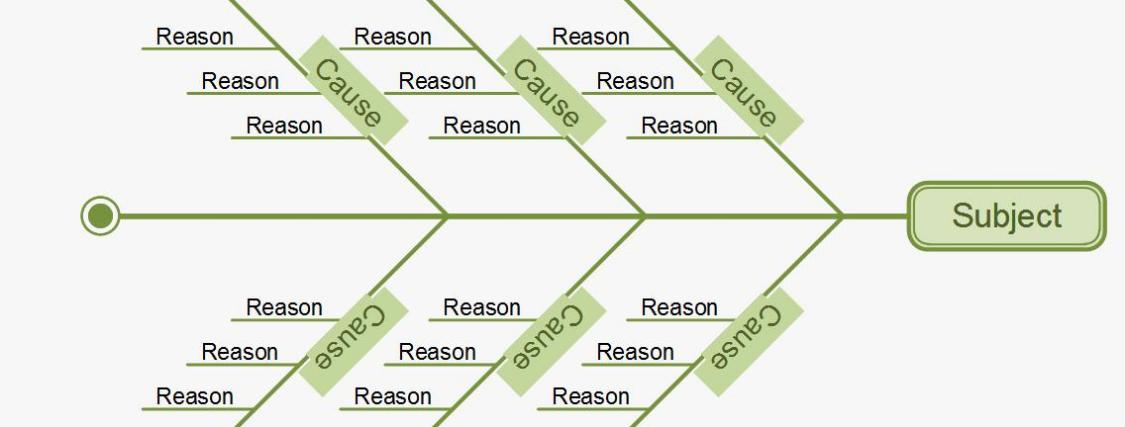
\includegraphics[width=0.90\textwidth]{root.cause.1.jpg}
%        \caption{}
    \end{figure}
\end{frame}


\begin{frame}{}
    \begin{figure}
        \centering
        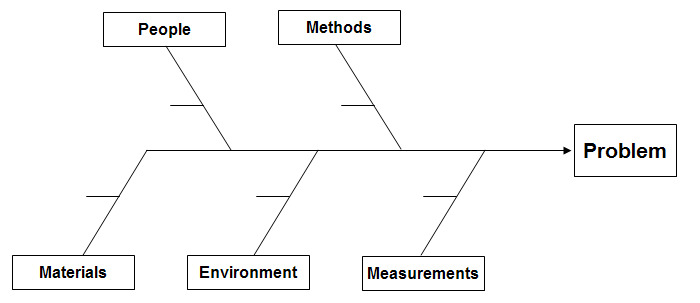
\includegraphics[width=0.90\textwidth]{root.cause.2.jpg}
%        \caption{}
    \end{figure}
\end{frame}


\begin{frame}{}
    \begin{figure}
        \centering
        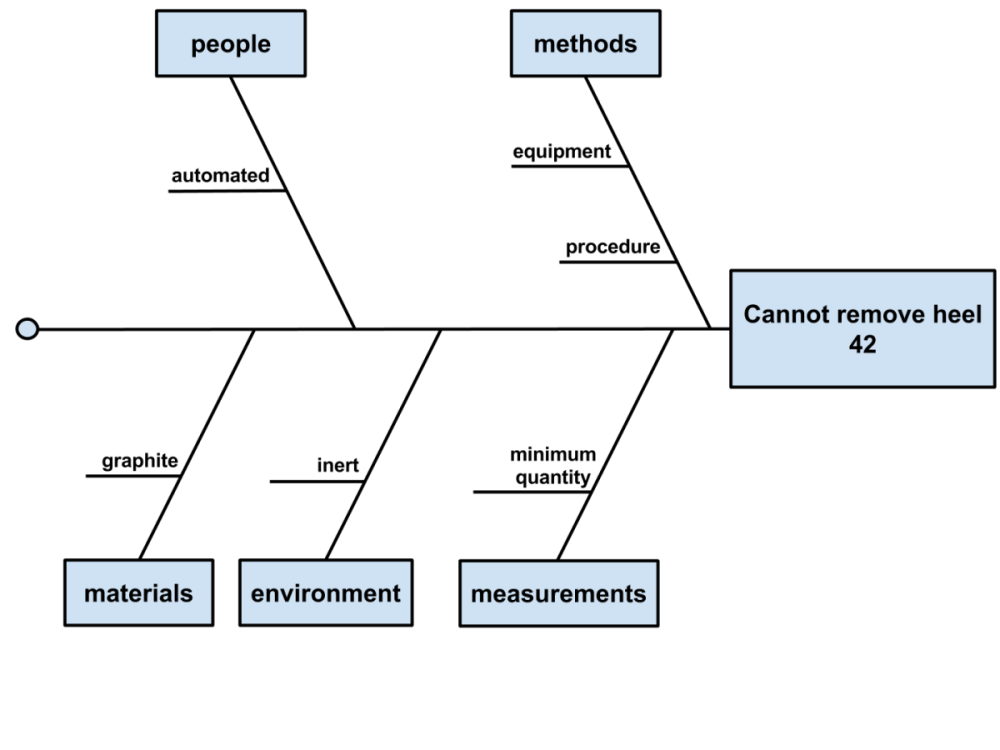
\includegraphics[width=0.90\textwidth]{fuel.fabrication.root.cause.jpg}
%        \caption{}
    \end{figure}
\end{frame}


\begin{frame}{Causes to make the metal stick to the crucible and cannot remove it cleanly}
    \begin{enumerate}[series=outerlist,topsep=0pt,itemsep=5pt,leftmargin=*,label=(\arabic*)]
        \item[]Graphite is the wrong material  
        \item[]Inert atmosphere
        \item[]Can induce vacuum
        \item[]Maybe there has to be X grams of it before removing  
        \item[]We also have to be able to detect the material in the crucible
        \item[]If the process is automated, it may be too complicated   
        \item[]Human hands might be needed  
        \item[]The removal process might need redesigning or optimization
        \item[]Maybe heat the crucible and pour metal into separate container
        \item[]Should be conducted by a team and be more in depth
    \end{enumerate}
\end{frame}


\begin{frame}[plain]{}
    \centering\LARGE\textbf{Mitigation}
\end{frame}


\addtocounter{framenumber}{-1}
\begin{frame}{Take action to eliminate or reduce the \acs{rpn}}
    \begin{enumerate}[series=outerlist,topsep=0pt,itemsep=7pt,leftmargin=*,label=(\arabic*)]
        \item[]Decrease likelihood of occurrence
        \item[]Decrease the severity of effects
        \item[]Lab-scale testing of different crucible materials may show a preferable material  
        \item[]May also show that removal cannot be achieved unless there is 100 grams, etc.
        \item[]Probably have a lot of crucibles on hand and maybe develop a clean, swap out procedure  
        \item[]May also show that removal cannot be achieved unless there is 100 grams, etc.
        \item[]My expert opinion would be that the crucible is the primary root cause
    \end{enumerate}
\end{frame}


\begin{frame}{Apply a `Plan-Do-Study-Act' approach}
    \begin{enumerate}[series=outerlist,topsep=0pt,itemsep=3pt,leftmargin=*,label=(\arabic*)]
        \item[]\textbf{What are we trying to accomplish?}
        \item[]Remove the heel without having it stick on the crucible  
        \item[]We have to measure the special nuclear material
        \item[]Then maybe store it and recycle it back into the melter
            \vspace{0.10in}
        \item[]\textbf{How will we know that a change is an improvement?}
        \item[]Heel is removed cleanly  
        \item[]Probably need to conduct lab scale experiments 
            \vspace{0.10in}
        \item[]\textbf{What changes can we make that will result in an improvement?}
        \item[]See fishbone discussion  
        \item[]Change material, procedures, environment  
            \vspace{0.10in}
        \item[]Iterative process -- but only so many meetings and brainstorming; at some point you have to get the job done
    \end{enumerate}
\end{frame}


\begin{frame}[plain]{}
    \begin{figure}
        \centering
        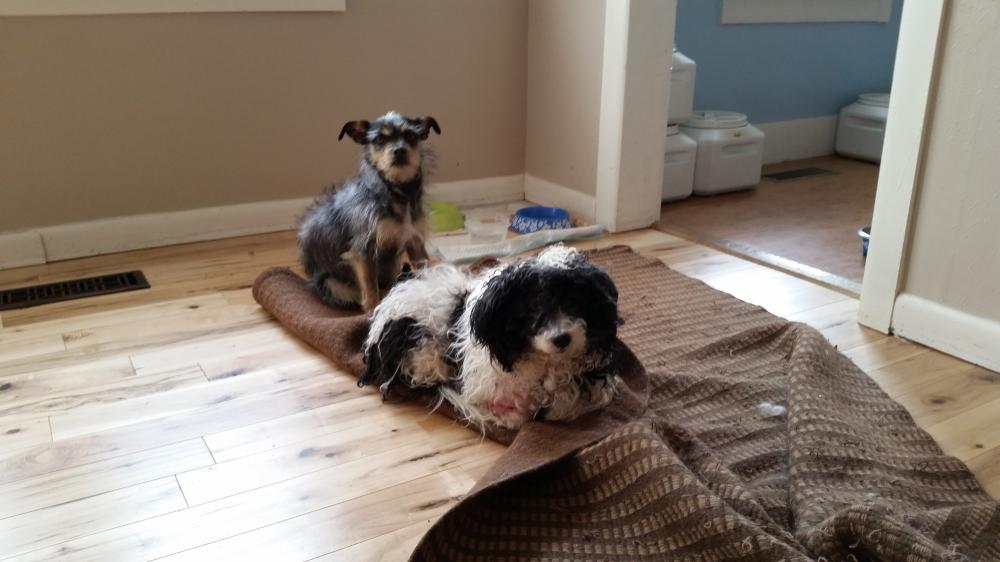
\includegraphics[width=0.65\textwidth]{final.jpg}
%        \caption{}
    \end{figure}
\end{frame}


%%%%%%%
%\begin{frame}{}
%    \begin{columns}
%
%        \begin{column}{0.50\textwidth}
%            \begin{enumerate}[series=outerlist,topsep=0pt,itemsep=21pt,leftmargin=*,label=(\arabic*)]
%                \item[]
%                \item[]
%            \end{enumerate}
%        \end{column}
%
%        \begin{column}{0.50\textwidth}
%            \begin{enumerate}[series=outerlist,topsep=0pt,itemsep=21pt,leftmargin=*,label=(\arabic*)]
%                \item[]
%                \item[]
%            \end{enumerate}
%        \end{column}
%
%    \end{columns}
%\end{frame}

%    \begin{figure}
%        \centering
%        \includegraphics[width=0.75\textwidth]{wsc.png}
%        \caption{\acs{wsc}}
%    \end{figure}


%\begin{frame}{References}
%    \bibliographystyle{nsf}
%    \footnotesize
%    \bibliography{references}
%\end{frame}
%%%%%%%


\end{document}
